%Galera_counter_example_original.tex



\documentclass{standalone}
% newcommands.tex

\newcommand{\enq}{\texttt{enq}}
\newcommand{\deq}{\texttt{deq}}
\newcommand{\pput}{\texttt{PUT}}
\newcommand{\get}{\texttt{GET}}
\newcommand{\vs}{\texttt{vis}}
\newcommand{\so}{\texttt{so}}
\newcommand{\arb}{\texttt{ar}}
\newcommand{\rf}{\texttt{rf}}

% example
\newcommand{\po}[2]{\draw [->, thick] (#1) to node[above] {\Large{\so}} (#2);}
\newcommand{\pva}[2]{\draw [->, thick] (#1) to node[above] {$\Large{\so},\Large{\vs},\Large{\arb}$} (#2);}
\newcommand{\pbva}[2]{\draw [->, thick] (#1) to node[above] {$\Large{\so}$} node[below] {$\Large{\vs},\Large{\arb}$} (#2);}
\newcommand{\pv}[2]{\draw [->, thick] (#1) to node[above] {\Large{\so}} node[below] {\Large{\vs}} (#2);}
\newcommand{\evis}[2]{\draw [->, thick] (#1) to node[above, sloped, near end] {\Large{\vs}} (#2);}
\newcommand{\mvis}[2]{\draw [->, thick] (#1) to node[above, sloped] {\Large{\vs}} (#2);}
\newcommand{\ar}[2]{\draw [->, thick, allow upside down] (#1) to node[above, sloped] {\Large{\arb}} (#2);}
\newcommand{\va}[2]{\draw [->, thick, allow upside down] (#1) to node[above, sloped] {$\Large{\vs},\Large{\arb}$} (#2);}
\newcommand{\vab}[2]{\draw [->, thick, allow upside down] (#1) to node[below, sloped, near end] {$\Large{\vs},\Large{\arb}$} (#2);}
\newcommand{\vae}[2]{\draw [->, thick, allow upside down] (#1) to node[above, sloped, near end] {$\Large{\vs},\Large{\arb}$} (#2);}
\newcommand{\vas}[2]{\draw [->, thick, allow upside down] (#1) to node[sloped, near start, above] {$\Large{\vs},\Large{\arb}$} (#2);}

% serialization
\newcommand{\scc}[2]{\draw [->, very thick] (#1) to (#2);}
\newcommand{\rva}[2]{\draw [->, thick, allow upside down] (#1) to node[above, sloped] {$\Large{\rf},\Large{\vs},\Large{\arb}$} (#2);}
\newcommand{\rvb}[2]{\draw [->, thick, allow upside down] (#1) to node[below, sloped] {$\Large{\rf},\Large{\vs},\Large{\arb}$} (#2);}


\usepackage{tikz}
\usetikzlibrary{shapes, positioning, arrows.meta, decorations.pathmorphing}

\begin{document}

    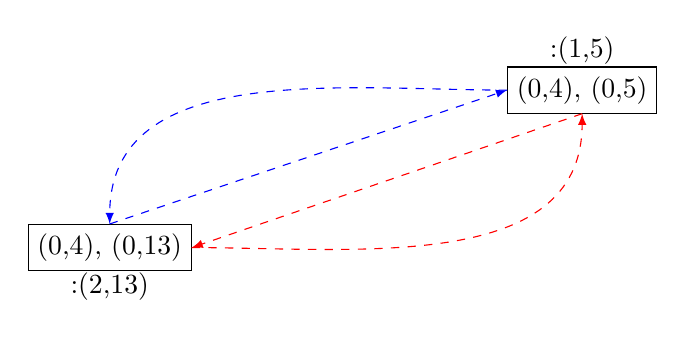
\begin{tikzpicture}[model/.style = {draw, minimum size = 15pt},  node distance = 0.5cm and 1.5cm]
        \node[model] (15) at (6,2) {$\R$(0,4), $\W$(0,5)};
        \node (textof15) at (6,2.5) {$\T$:(1,5)};
        \node[model] (213) at (0,0) {$\R$(0,4), $\W$(0,13)};
        \node (textof213) at (0,-0.5) {$\T$:(2,13)};
        %\node[model] (14) at (6,0) {Read(0,5)};
        %\node (textof14) at (6,-0.5) {Txn:(1,4)};
        \path[dashed, -latex, color=red] (15.south) edge node[above] {$\WW$} (213.east); 
        \path[dashed, -latex, color=blue] (213.north) edge node[below] {$\WW$} (15.west); 
        \path[dashed, -latex, color=blue] (15.west) edge [out=180,in=90] node[above] {$\RW$} (213.north);
        \path[dashed, -latex, color=red] (213.east) edge [out=0,in=-90] node[above] {$\RW$} (15.south);
        %\path[dashed, -latex,color=red] (14.west) edge node[below] {rw} (28.east); 
    \end{tikzpicture}

\end{document}